\section{Examples}

\label{sect:examples}

%\subsection{Socket Programming, with Exceptions}

The \texttt{ST} library can be used in any situation which calls for tracking
of the states of resource in types. In this section, we present several
diverse examples which
show how the library allows us to compose stateful systems both
horizontally (that is, using multiple stateful systems at once) and
vertically (that is, implementing one stateful system in terms of one or
more others). 

\subsection{A Graphics Interface}

Listing \ref{fig:drawiface} shows an interface for a small graphics library
which supports creating a window and drawing into that window.
The \texttt{flip} operation supports double buffering.
We create a state of type \texttt{Surface} using the following function:

\small
\begin{code}
initWindow : Int -> Int -> ST m (Maybe Var) [addIfJust Surface]
\end{code}
\normalsize

This uses a type level function \texttt{addIfJust}, provided by the \texttt{ST}
library, which allows us to write concisely in a type that the function will
add a resource when it successfully returns a variable:

\small
\begin{code}
addIfJust : Type -> Action (Maybe a)
addIfJust ty = Add (maybe [] (\var => [var ::: ty]))
\end{code}
\normalsize

\small
\begin{code}[float=h, frame=single,caption={The \texttt{Draw} interface which
supports drawing lines in a window},label=fig:drawiface]
interface Draw (m : Type -> Type) where
  Surface : Type

  initWindow : Int -> Int -> ST m (Maybe Var) [addIfJust Surface]
  closeWindow : (win : Var) -> ST m () [Remove win Surface] 
  flip : (win : Var) -> ST m () [win ::: Surface]
  filledRectangle : (win : Var) -> (Int, Int) -> (Int, Int) -> Col ->
                    ST m () [win ::: Surface]
  drawLine : (win : Var) -> (Int, Int) -> (Int, Int) -> Col ->
             ST m () [win ::: Surface]
\end{code}
\normalsize

We can provide an implementation for this interface using the SDL graphics
library\footnote{\url{https://www.libsdl.org/}}, for example:

\small
\begin{code}
implementation Draw IO where
  Surface = State SDLSurface
  ...
\end{code}
\normalsize

Having defined a primitive interface for graphics operations, we can use it
as a basis for more high level interfaces. For example, we can build a library
for turtle graphics by building a \emph{composite} resource from a
\texttt{Surface} and the state of a turtle (including location, direction and
pen colour).

\subsection{Turtle Graphics}

\label{sect:turtle}

Turtle graphics involves a ``turtle'' manoeuvring around a screen, drawing
lines as it moves. 
It has attributes describing its location, direction, and
pen colour. 
There are commands for moving the turtle forwards, turning through an angle,
and changing colour.
Listing~\ref{fig:turtleiface} gives one possible interface 
using \texttt{ST}.

\small
\begin{code}[float=h, frame=single,caption={An interface for turtle graphics,
supporting creating a turtle, drawing lines, and rendering the result},
label=fig:turtleiface]
interface TurtleGraphics (m : Type -> Type) where
  Turtle : Type

  start : Int -> Int -> ST m (Maybe Var) [addIfJust Turtle]
  end : (t : Var) -> ST m () [Remove t Turtle]
  fd : (t : Var) -> Int -> ST m () [t ::: Turtle]
  rt : (t : Var) -> Int -> ST m () [t ::: Turtle]
  col : (t : Var) -> Col -> ST m () [t ::: Turtle]
  render : (t : Var) -> ST m () [t ::: Turtle]
\end{code}
\normalsize

The \texttt{start} function initialises the system with window dimensions. 
Then, the state of the
turtle can be updated by issuing commands. Finally, the \texttt{render}
function displays the picture drawn so far in a window. The following
function, for example, initialises a turtle and, if successful, draws a
coloured square:

\small
\begin{code}
square : (ConsoleIO m, TurtleGraphics m) => ST m () []
square = do Just t <- start 640 480 | Nothing => putStr "Can't make turtle\n"
            col t yellow; fd t 100; rt t 90; col t green; fd t 100; rt t 90
            col t red; fd t 100; rt t 90; col t blue; fd t 100; rt t 90
            render t; end t
\end{code}
\normalsize

We can implement the interface using \texttt{Draw}, and render using
a \texttt{Surface} but we need additional state to represent the current
state of the turtle, and to record what we need to draw when \texttt{render}
is called. We can achieve this using a composite resource:

\small
\begin{code}
implementation Draw m => TurtleGraphics m where
  Turtle = Composite [Surface {m}, State Col, State (Int, Int, Int), 
                      State (List Line)] 
  ...
\end{code}
\normalsize

The components are: the \texttt{Surface} to draw on; the current pen colour,
the current turtle location and direction, and a list
of lines to draw. When we initialise the system, we create each component
of the composite resource then \texttt{combine} them:
  
\small
\begin{code}
start x y = do Just srf <- initWindow x y | Nothing => pure Nothing
               col <- new white; pos <- new (320, 200, 0)
               lines <- new []; turtle <- new ()
               combine turtle [srf, col, pos, lines]
               pure (Just turtle)
\end{code}
\normalsize

In each operation, to access an individual element of the composite resource,
we need to \texttt{split} the resource, then \texttt{combine} the components
when done. For example, to turn right:

\small
\begin{code}
rt t angle = do [srf, col, pos, lines] <- split t
                (x, y, d) <- read pos
                write pos (x, y, d + angle `mod` 360)
                combine t [srf, col, pos, lines]
\end{code}
\normalsize

In this way, we can implement a larger system as a \emph{hieararchy} of
smaller systems. The \texttt{Turtle}, as far as the programmer who writes
\texttt{square} is concerned, is an individual system, but internally there
are state machines all the way down to the concrete implementations of
\texttt{Draw} and \texttt{State}.

\subsection{Socket Programming, with Error Handling}

\begin{tabular}{ll}
\begin{minipage}{9cm}
The POSIX sockets API supports communication between processes across
a network. A \emph{socket} represents an endpoint of a network communication,
and can be in one of several states: \texttt{Ready}, the initial state;
\texttt{Bound}, meaning that it has been bound to an address ready for incoming
connections; \texttt{Listening}, meaning that it is listening for incoming
connections; \texttt{Open}, meaning that it is ready for sending and
receiving data; and \texttt{Closed} meaning that it is no longer active.
The diagram on the right shows how the operations provided by the API
modify the state, where \texttt{Ready} is the initial state.
\end{minipage}
&
\begin{minipage}{6.5cm}
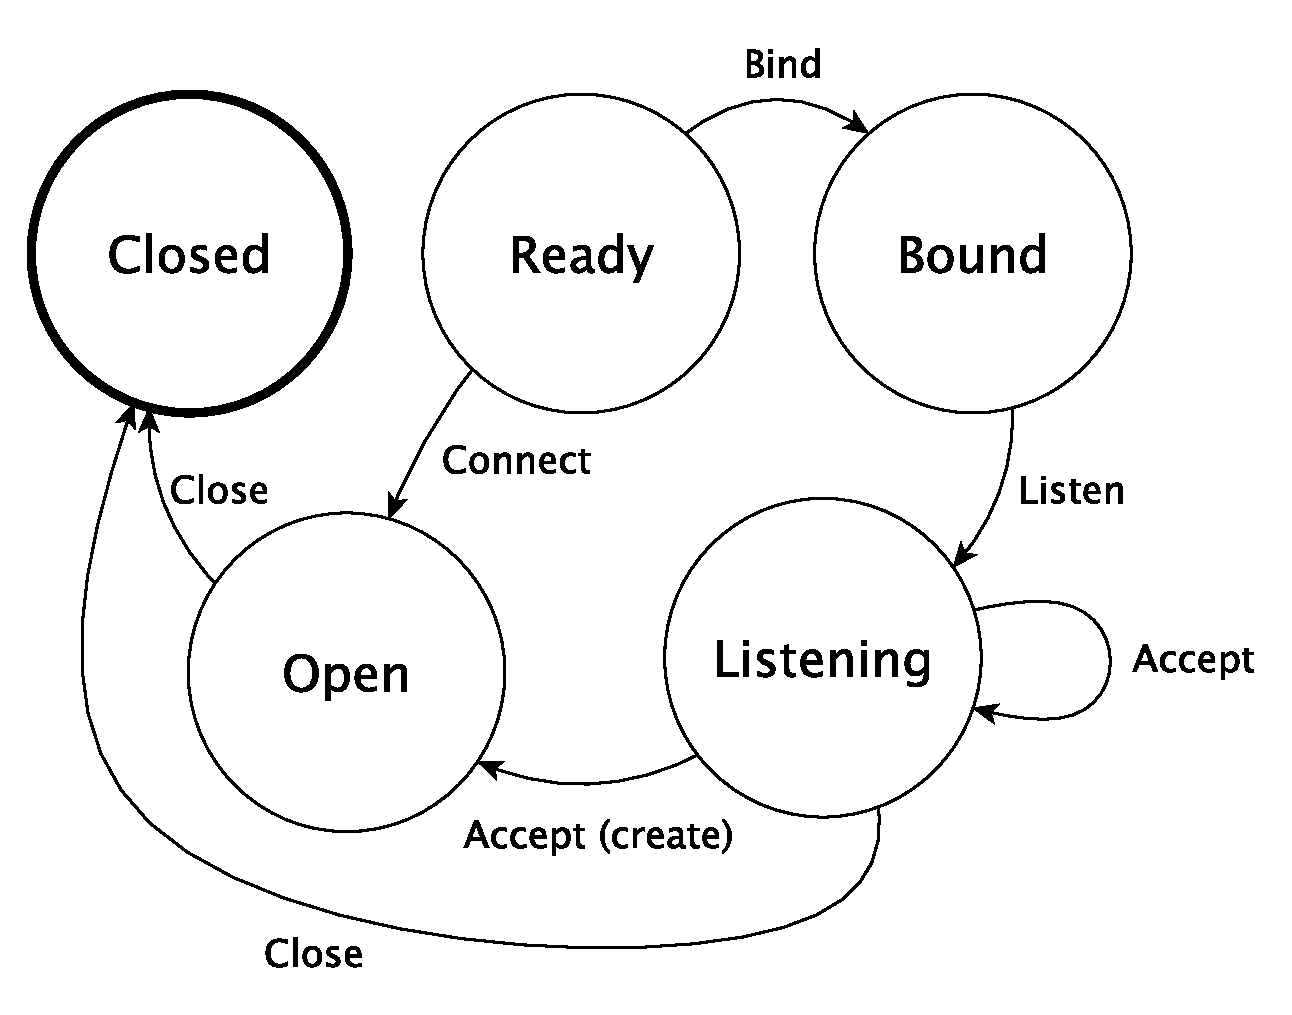
\includegraphics[width=6.5cm]{diagrams/netstate.pdf}
\end{minipage}
\end{tabular}

\small
\begin{code}[float=h, frame=single,caption={The POSIX sockets API, written
as in interface for \texttt{ST} describing how each operation affects
socket state},
label=fig:socketsiface]
data SocketState = Ready | Bound | Listening | Open | Closed

interface Sockets (m : Type -> Type) where
  Sock : SocketState -> Type

  socket : SocketType -> ST m (Either () Var) [addIfRight (Sock Ready)]
  bind : (sock : Var) -> (addr : Maybe SocketAddress) -> (port : Port) ->
    ST m (Either () ()) [sock ::: Sock Ready :-> (Sock Closed `or` Sock Bound)]
  listen : (sock : Var) ->
    ST m (Either () ()) [sock ::: Sock Bound :-> (Sock Closed `or` Sock Listening)]
  accept : (sock : Var) ->
    ST m (Either () Var) [addIfRight (Sock Open), sock ::: Sock Listening]
  connect : (sock : Var) -> SocketAddress -> Port ->
    ST m (Either () ()) [sock ::: Sock Ready :-> (Sock Closed `or` Sock Open)]
  close : (sock : Var) -> {auto prf : CloseOK st} ->
    ST m () [sock ::: Sock st :-> Sock Closed]
  remove : (sock : Var) -> ST m () [Remove sock (Sock Closed)]
  send : (sock : Var) -> String -> 
    ST m (Either () ()) [sock ::: Sock Open :-> (Sock Closed `or` Sock Open)]
  recv : (sock : Var) ->
    ST m (Either () String) [sock ::: Sock Open :-> (Sock Closed `or` Sock Open)]
\end{code}
\normalsize

Listing~\ref{fig:socketsiface} shows how these operations can be given precise
types which describe how the operations affect socket state, using \texttt{ST}.
By convention, each operation returns something with a type of the form
\texttt{Either a b}, representing the possibility of failure.
The \texttt{ST} library provides two helper functions
which allow us to write concise types for these operations:

\small
\begin{code}
addIfRight : Type -> Action (Either a b)
addIfRight ty = Add (either (const []) (\var => [var ::: ty]))

or : a -> a -> Either b c -> a
or x y = either (const x) (const y)
\end{code}
\normalsize

Note, in particular, that \texttt{accept} explicitly creates a new
\texttt{Open} socket specifically for processing an incoming connection,
keeping the existing socket in a \texttt{Listening} state. This could allow,
for example, processing an incoming connection in a different thread:

\small
\begin{code}
accept : (sock : Var) ->
    ST m (Either () Var) [addIfRight (Sock Open), sock ::: Sock Listening]
\end{code}
\normalsize

We could use \texttt{Sockets} to write an ``echo'' server which repeatedly
accepts an incoming connection from a client, and echoes a message back to the
client. We can define a function \texttt{echoServer} which accepts connections
on a \texttt{Listening} socket, and logs messages to the console:

\small
\begin{code}
echoServer : (ConsoleIO m, Sockets m) => (sock : Var) -> 
             ST m () [Remove sock (Sock {m} Listening)]
\end{code}
\normalsize

Then, before we start up \texttt{echoServer}, we need to create a socket, bind
it to a port, then begin listening for incoming connections. Each of these
operations could fail, so we include pattern matching alternatives to clean
up the resources if necessary:

\small
\begin{code}
startServer : (ConsoleIO io, Sockets io) => ST io () [] 
startServer = do Right sock <- socket Stream        | Left err => pure () 
                 Right ok <- bind sock Nothing 9442 | Left err => remove sock
                 Right ok <- listen sock            | Left err => remove sock
                 echoServer sock
\end{code}
\normalsize

We can begin writing \texttt{echoServer} as follows, accepting a connection
or cleaning up the resources and returning if \texttt{accept} fails:

\small
\begin{code}
echoServer sock = 
  do Right new <- accept sock | Left err => do close sock; remove sock
     ?rest
\end{code}
\normalsize

Checking the type of \texttt{?rest} here shows us that we have a 
\texttt{new} socket, which is \texttt{Open} and therefore ready to communicate
with the client, as well as \texttt{sock} which remains listening for new
connections:

\small
\begin{code}
rest : STrans m () [new ::: Sock Open, sock ::: Sock Listening]
                   (\result1 => [])
\end{code}
\normalsize

\subsection{Asynchronous Programming with Threads}

\label{sect:async}

In \texttt{ST}, resources are linear, in that there is exactly one reference
to each, and once a resource has been overwritten the old value is no longer
available. So, if we spawn a thread, we need to consider how to preserve
linearity, and maintain only one reference to each resource.
Listing~\ref{fig:asynciface} shows one way to do this, where the
\texttt{fork} function takes a thread described in \texttt{STrans}, and
a proof that the forked thread uses a subcontext of the parent thread.
Then, the parent thread keeps only the resources which are not used by
the child thread.

\small
\begin{code}[float=h, frame=single,caption={An interface supporting
asynchronous programming, dividing resources between a child
and a parent thread},
label=fig:asynciface]
interface Conc (m : Type -> Type) where
  fork : (thread : STrans m () thread_res (const [])) ->
         {auto tprf : SubCtxt thread_res all} ->
         STrans m () all (const (kept tprf)) 
\end{code}
\normalsize

An implementation of \texttt{Conc} then needs to divide the resources
appropriately. We can achieve this with \texttt{dropSubCtxt} (to remove
the subcontext from the current thread, returning the environment) and
\texttt{runWith} (to pass that environment to the spawned thread):

\small
\begin{code}
implementation Conc IO where
  fork thread = do threadEnv <- dropSubCtxt
                   lift (spawn (do runWith threadEnv thread
                                   pure ()))
                   pure ()

\end{code}
\normalsize

The Idris library defines \texttt{spawn} to create a new thread. It
returns a process identifier, to allow communication between threads, but
we leave communication between threads for future work.

\subsection{Managing Sessions: A Random Number Server}

\label{sect:randserver}

In the turtle graphics example, we implemented a high level
graphics API in terms of lower level drawing operations. Similarly, we can
implement a high level network application protocol in terms of sockets.
Listing~\ref{fig:randiface} shows an interface for a server which replies
to requests from a client for a random number within a bound. 

\small
\begin{code}[float=h, frame=single,caption={An interface for a server which
returns random numbers within a given bound},
label=fig:randiface]
data SessionState = Waiting | Processing | Done

interface RandomSession (m : Type -> Type) where
  Connection : SessionState -> Type
  Server : Type

  recvReq : (conn : Var) ->
    ST m (Maybe Integer) [conn ::: Connection Waiting :->
                           \res => Connection (case res of
                                                    Nothing => Done
                                                    Just _ => Processing)]
  sendResp : (conn : Var) -> Integer ->
             ST m () [conn ::: Connection Processing :-> Connection Done]
  start : ST m (Maybe Var) [addIfJust Server]
  quit : (srv : Var) -> ST m () [Remove srv Server]
  done : (conn : Var) -> ST m () [Remove conn (Connection Done)]
  accept : (srv : Var) ->
           ST m (Maybe Var) [srv ::: Server, addIfJust (Connection Waiting)]
\end{code}
\normalsize

The interface defines two types:

\begin{itemize}
\item \texttt{Connection}, which is the current state of a session with
a client. A session is either \texttt{Waiting} for the client to send
a request, \texttt{Processing} the request from the client, or \texttt{Done}
and ready to close.
\item \texttt{Server}, which is the type of a server which processes
incoming client requests.
\end{itemize}

Overall, a server listens for an incoming request from a client, 
and when it receives a request, it initialises a session with the client
and continues waiting for further incoming requests. In a session, we can
call one of:

\begin{itemize}
\item \texttt{recvReq}, which, if we're in the \texttt{Waiting} state,
receives a request from a client, and if it is valid moves into the
\texttt{Processing} state.
\item \texttt{sendResp}, which, if we're in the \texttt{Processing} state,
sends a random number within the given bound. Note that \texttt{sendResp}
itself is intended to do the work of generating the random number.
\item \texttt{done}, which closes the session and removes the \texttt{Connection}
state.
\end{itemize}

To implement a random number server, we'll use this interface, as well
as \texttt{ConsoleIO} for console logging, and \texttt{Conc} to process
requests asynchronously. To avoid repetition in every function signature,
Idris provides a notation to allow us to state that every function in a
block is constrained by the same interfaces:

\small
\begin{code}
using (ConsoleIO m, RandomSession m, Conc m)
\end{code}
\normalsize

We implement a session with \texttt{rndSession} which, given a
\texttt{Connection} in the \texttt{Waiting} state will process a client
request and eventually delete the connection, using \texttt{recvReq},
\texttt{sendResp} and \texttt{done}:

\small
\begin{code}
rndSession : (conn : Var) -> ST m () [Remove conn (Connection {m} Waiting)]
\end{code}
\normalsize

The main loop of the server calls \texttt{accept} to receive an incoming
connection. If it fails, it reports an error. Otherwise, it uses
\texttt{fork} to process the incoming connection in a separate thread.
The resources are divided between \texttt{rndSession} (whose type states that
it receives the \texttt{Connection} variable \texttt{conn}) and the parent thread, which
retains the \texttt{Server} variable \texttt{srv}:

\small
\begin{code}
rndLoop : (srv : Var) -> ST m () [srv ::: Server {m}]
rndLoop srv = do Just conn <- accept srv | Nothing => putStr "accept failed\n"
                 putStr "Connection received\n"
                 fork (rndSession conn)
                 rndLoop srv
  
rndServer : ST m () []
rndServer = do Just srv <- start | Nothing => putStr "Can't start server\n"
               rndLoop srv; quit srv
\end{code}
\normalsize

Finally, we can implement the interface using composite resources for both
the \texttt{Connection} and the \texttt{Server}. Each one carries an
\texttt{Integer} seed for the random number generator, and a socket for
receiving incoming connections. In the case of \texttt{Connection}, the socket
will be in a different state depending on the current state of the session. In
particular, once the session is \texttt{Done}, the socket will need to be
\texttt{Closed}.

\small
\begin{code}
implementation (ConsoleIO m, Sockets m) => RandomSession m where
  Connection Waiting = Composite [State Integer, Sock {m} Open]
  Connection Processing = Composite [State Integer, Sock {m} Open]
  Connection Done = Composite [State Integer, Sock {m} Closed]
  Server = Composite [State Integer, Sock {m} Listening]
  ...
\end{code}
\normalsize

% The complete code for this and the previous examples is available as
% supplementary material, and will be made available online.
